\documentclass[aspectratio=169,
				xcolor=table]{beamer}

% Load general definitions
\usepackage[utf8]{inputenc}
%\usepackage[T1]{fontenc}
\usepackage[brazil]{babel}
\usepackage{amsmath}
\usepackage{amsfonts}
\usepackage{amssymb}
\usepackage{graphicx}
\usepackage{verbatim}
\usepackage{cancel}
\usepackage{askmaps}
\usepackage{tabularx}
\usepackage[table]{xcolor}
%\usepackage{tikz}
\usepackage{multirow}
\usepackage{mathtools}
\usepackage{color, colortbl}
\usepackage{etoolbox}
\usepackage{pbox}
\usepackage{changepage}
\usepackage{xpatch}
\usepackage{array}
\usepackage{marvosym}
\usepackage{tabu}
\usepackage{multicol}
\usepackage{listings}
\usepackage{underscore}
\usepackage{filecontents}
\usepackage[]{algorithm2e}
\usepackage{ragged2e}

\newcolumntype{P}[1]{>{\centering\arraybackslash}m{#1}}
\definecolor{Gray}{gray}{0.75}
\definecolor{Gray2}{gray}{0.85}

\definecolor{lightBlue}{HTML}{DAE8FC}
\definecolor{Blue}{RGB}{51, 51, 204}

%\useinnertheme[lily]{rounded}
\usetheme{UniEvangelica}
%\usetheme{Copenhagen}
%\usetheme{Berlin}
%\usecolortheme{dolphin}
\tolerance=1
\emergencystretch=\maxdimen
\hyphenpenalty=10000
\hbadness=10000

\setbeamertemplate{navigation symbols}{}%remove navigation symbols


\let\olditem=\item% 
\renewcommand{\item}{\olditem \justifying}%
\def\center{\trivlist \centering\item\relax}
\def\endcenter{\endtrivlist}

\setbeamertemplate{itemize/enumerate body begin}{\large}
\setbeamertemplate{itemize/enumerate subbody begin}{\large}

\setbeamertemplate{itemize item}{\raisebox{0.1ex}{$\blacktriangleright$}\hskip0.1em}
\setbeamertemplate{itemize subitem}{\raisebox{0.1ex}{$\blacktriangleright$}\hskip0.1em}

\newcommand{\greenarrow}{\textcolor{green}{\rotatebox[origin=c]{180}{\MVArrowDown}}}

\newcommand{\redarrow}{\textcolor{red}{\MVArrowDown}}

%\newcommand{\ftable}{
%	\begin{table}
%		\large
%		\centering
%		\rowcolors{1}{\ifnumless{\rownum}{2}{Blue}{lightBlue}}{}
%}

\newenvironment{eftable}{
	\begin{table}
		\large
		\centering
		\rowcolors{1}{}{Blue}
		\rowcolors{1}{\ifnumless{\rownum}{2}{Blue}{lightBlue}}{}
	}
	{
	\end{table}
}


%\setbeamertemplate{frametitle}
%{
%	%\vspace*{-2em}	
%	\insertframetitle
%
%	 %\textcolor{white}{\LARGE \insertframetitle}
%
%}

% Specific definitions
\institute[]{\uppercase{Engenharia de Software}}
\title[]{Sistemas Distribuídos}
\subtitle[]{\uppercase{Conceitos Básicos}}
\author[]{Prof. M.e Alexandre Tannus}
\date{}

%\AtBeginSection{\frame{\tableofcontents[currentsection]}}

\begin{document}
	\begin{frame}
		\titlepage		
	\end{frame}

	\begin{frame}
		\tableofcontents
	\end{frame}	

	\section{Introdução}
	\begin{frame}
		\frametitle{Definição}
		\begin{itemize}
			\item Rede
			\begin{itemize}
				\item Conjunto de entidades interligadas entre si
			\end{itemize}
		\end{itemize}
		\begin{figure}
			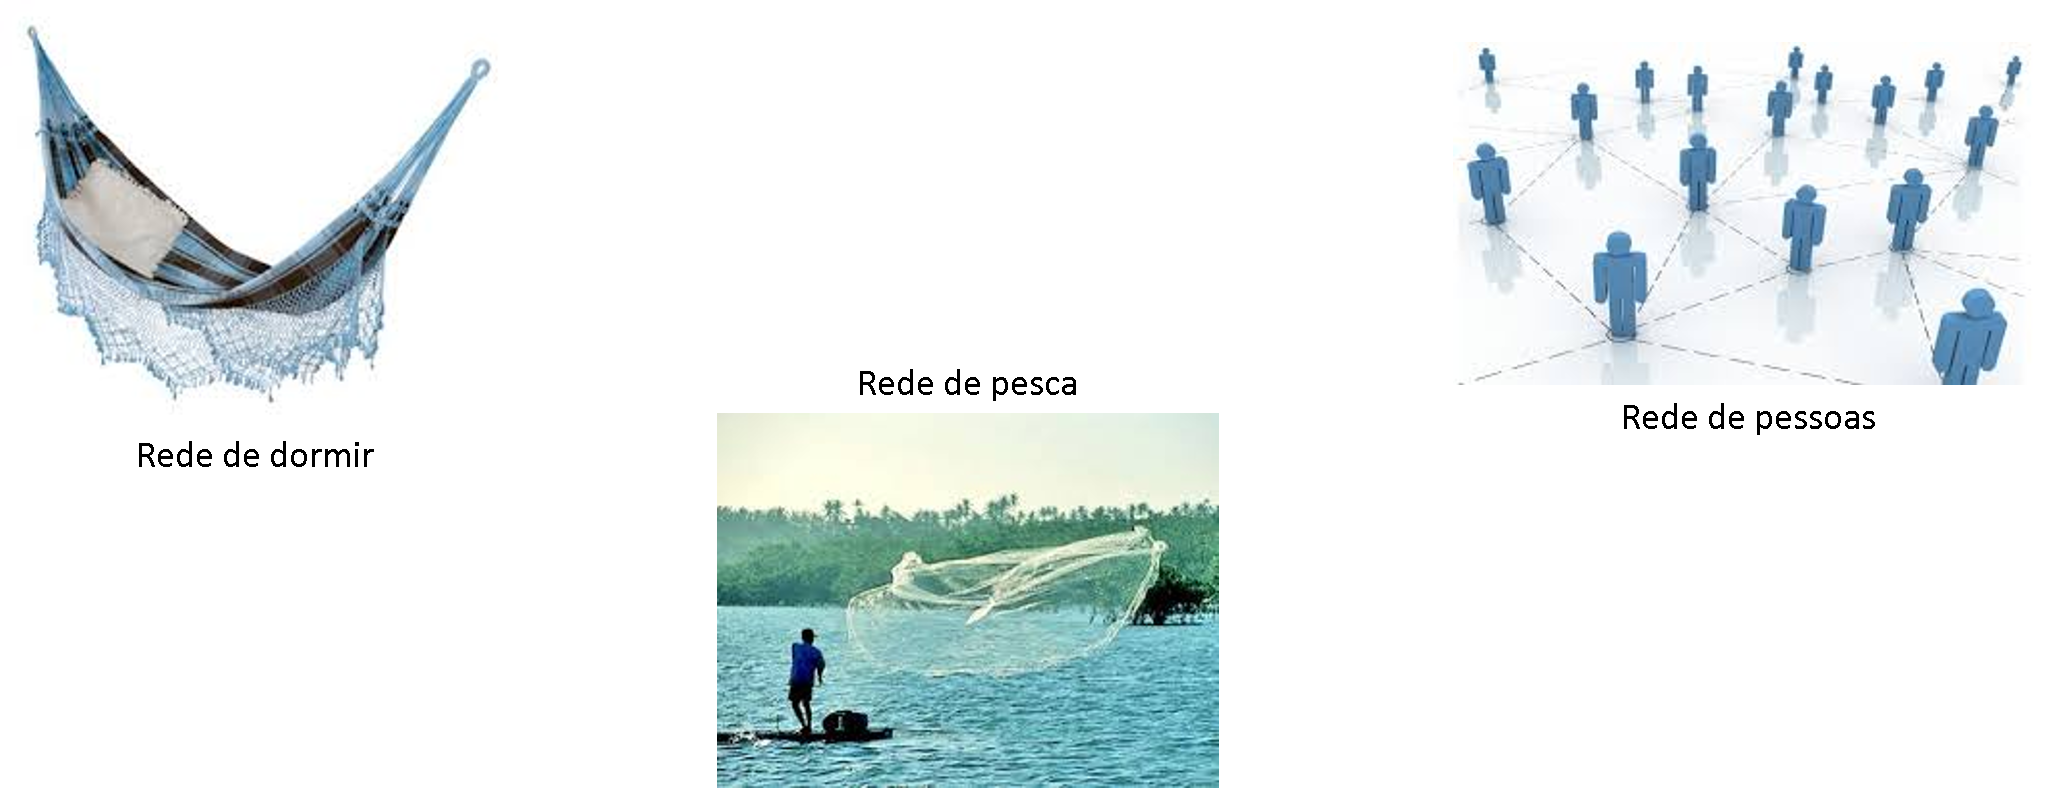
\includegraphics[height=4cm, keepaspectratio]{../figs/cap01/redes01.png} 
		\end{figure}
	\end{frame}

	\begin{frame}
		\frametitle{Definição}
		\begin{figure}
			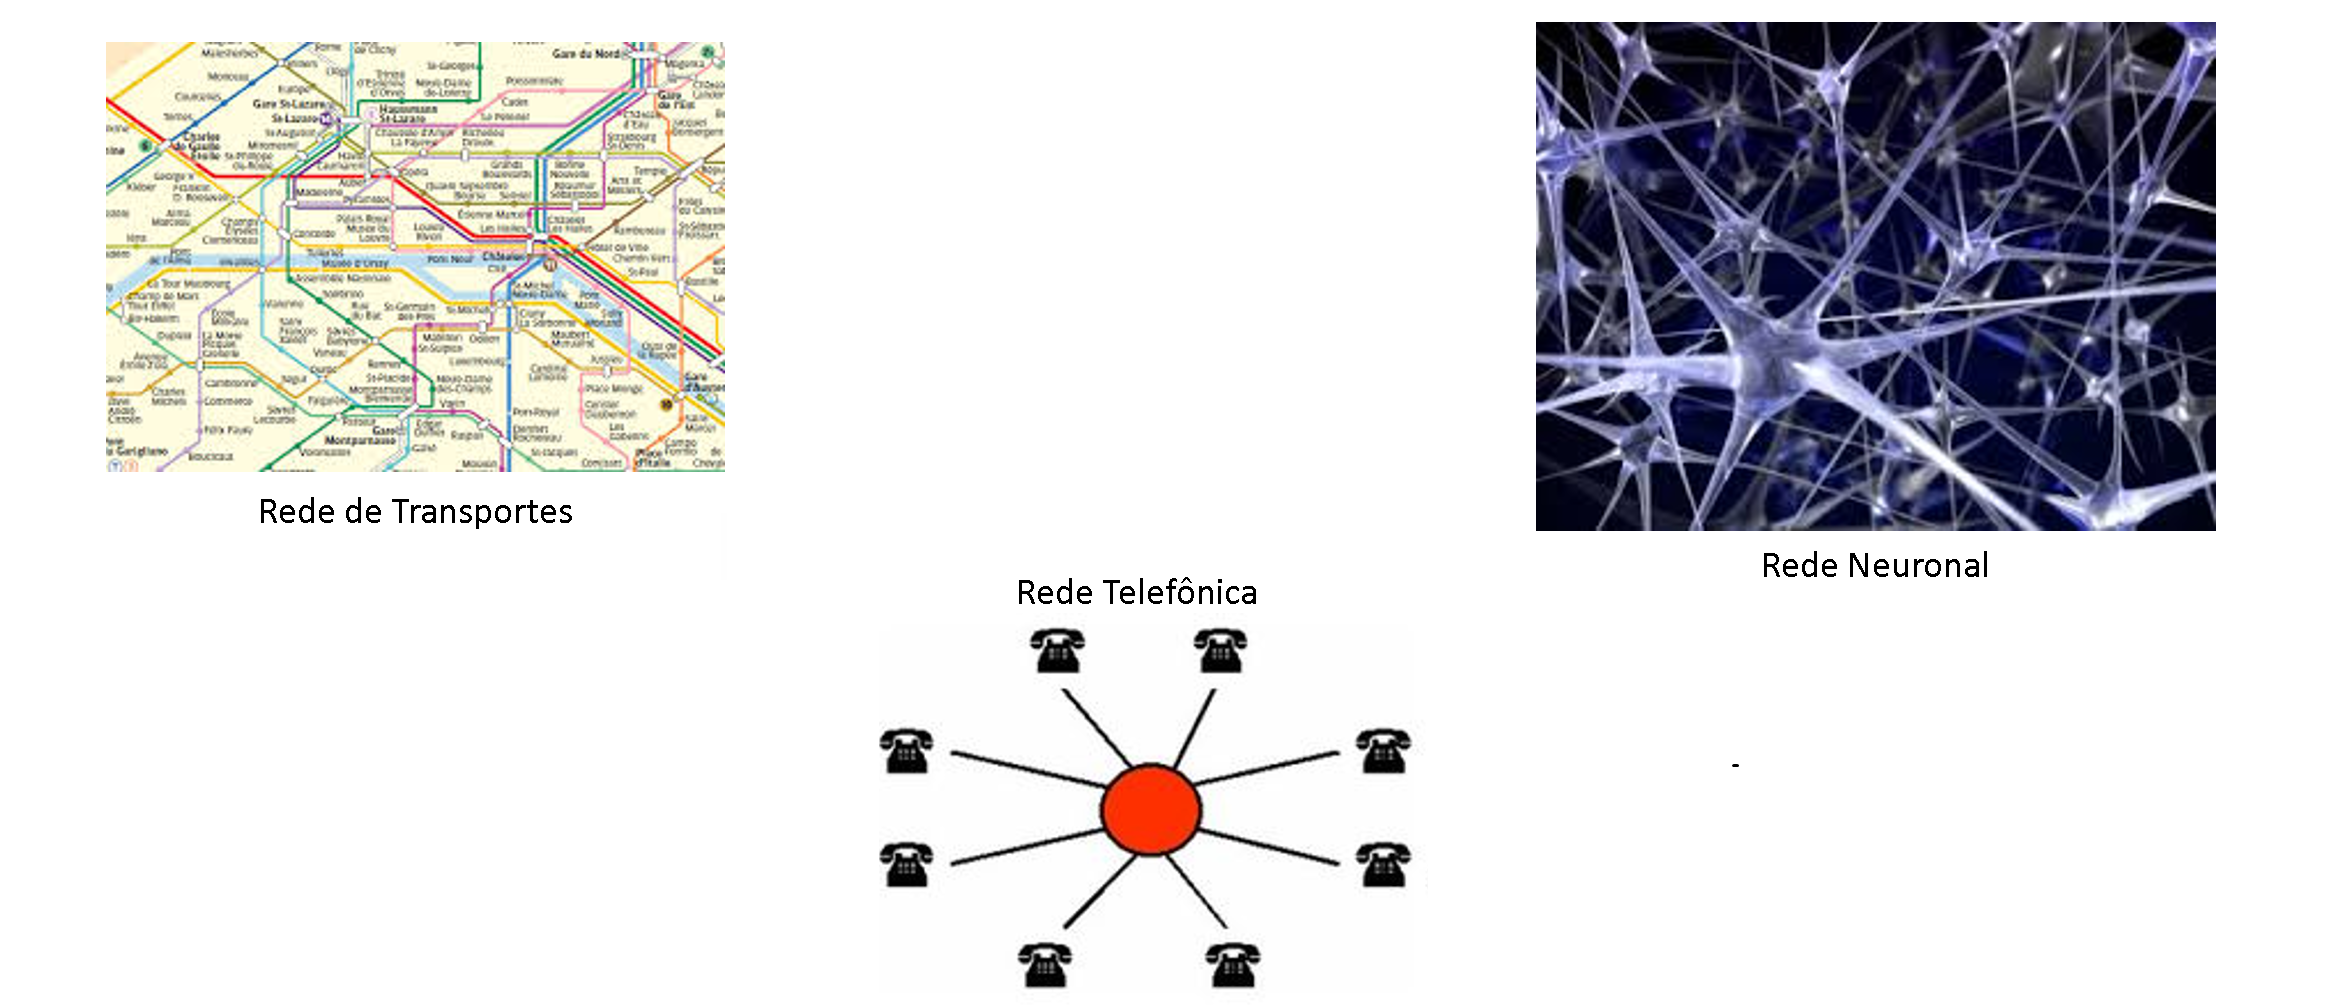
\includegraphics[height=5.5cm, keepaspectratio]{../figs/cap01/redes02.png} 
		\end{figure}
	\end{frame}	
	
	\begin{frame}
		\frametitle{Definição}
		\begin{figure}
			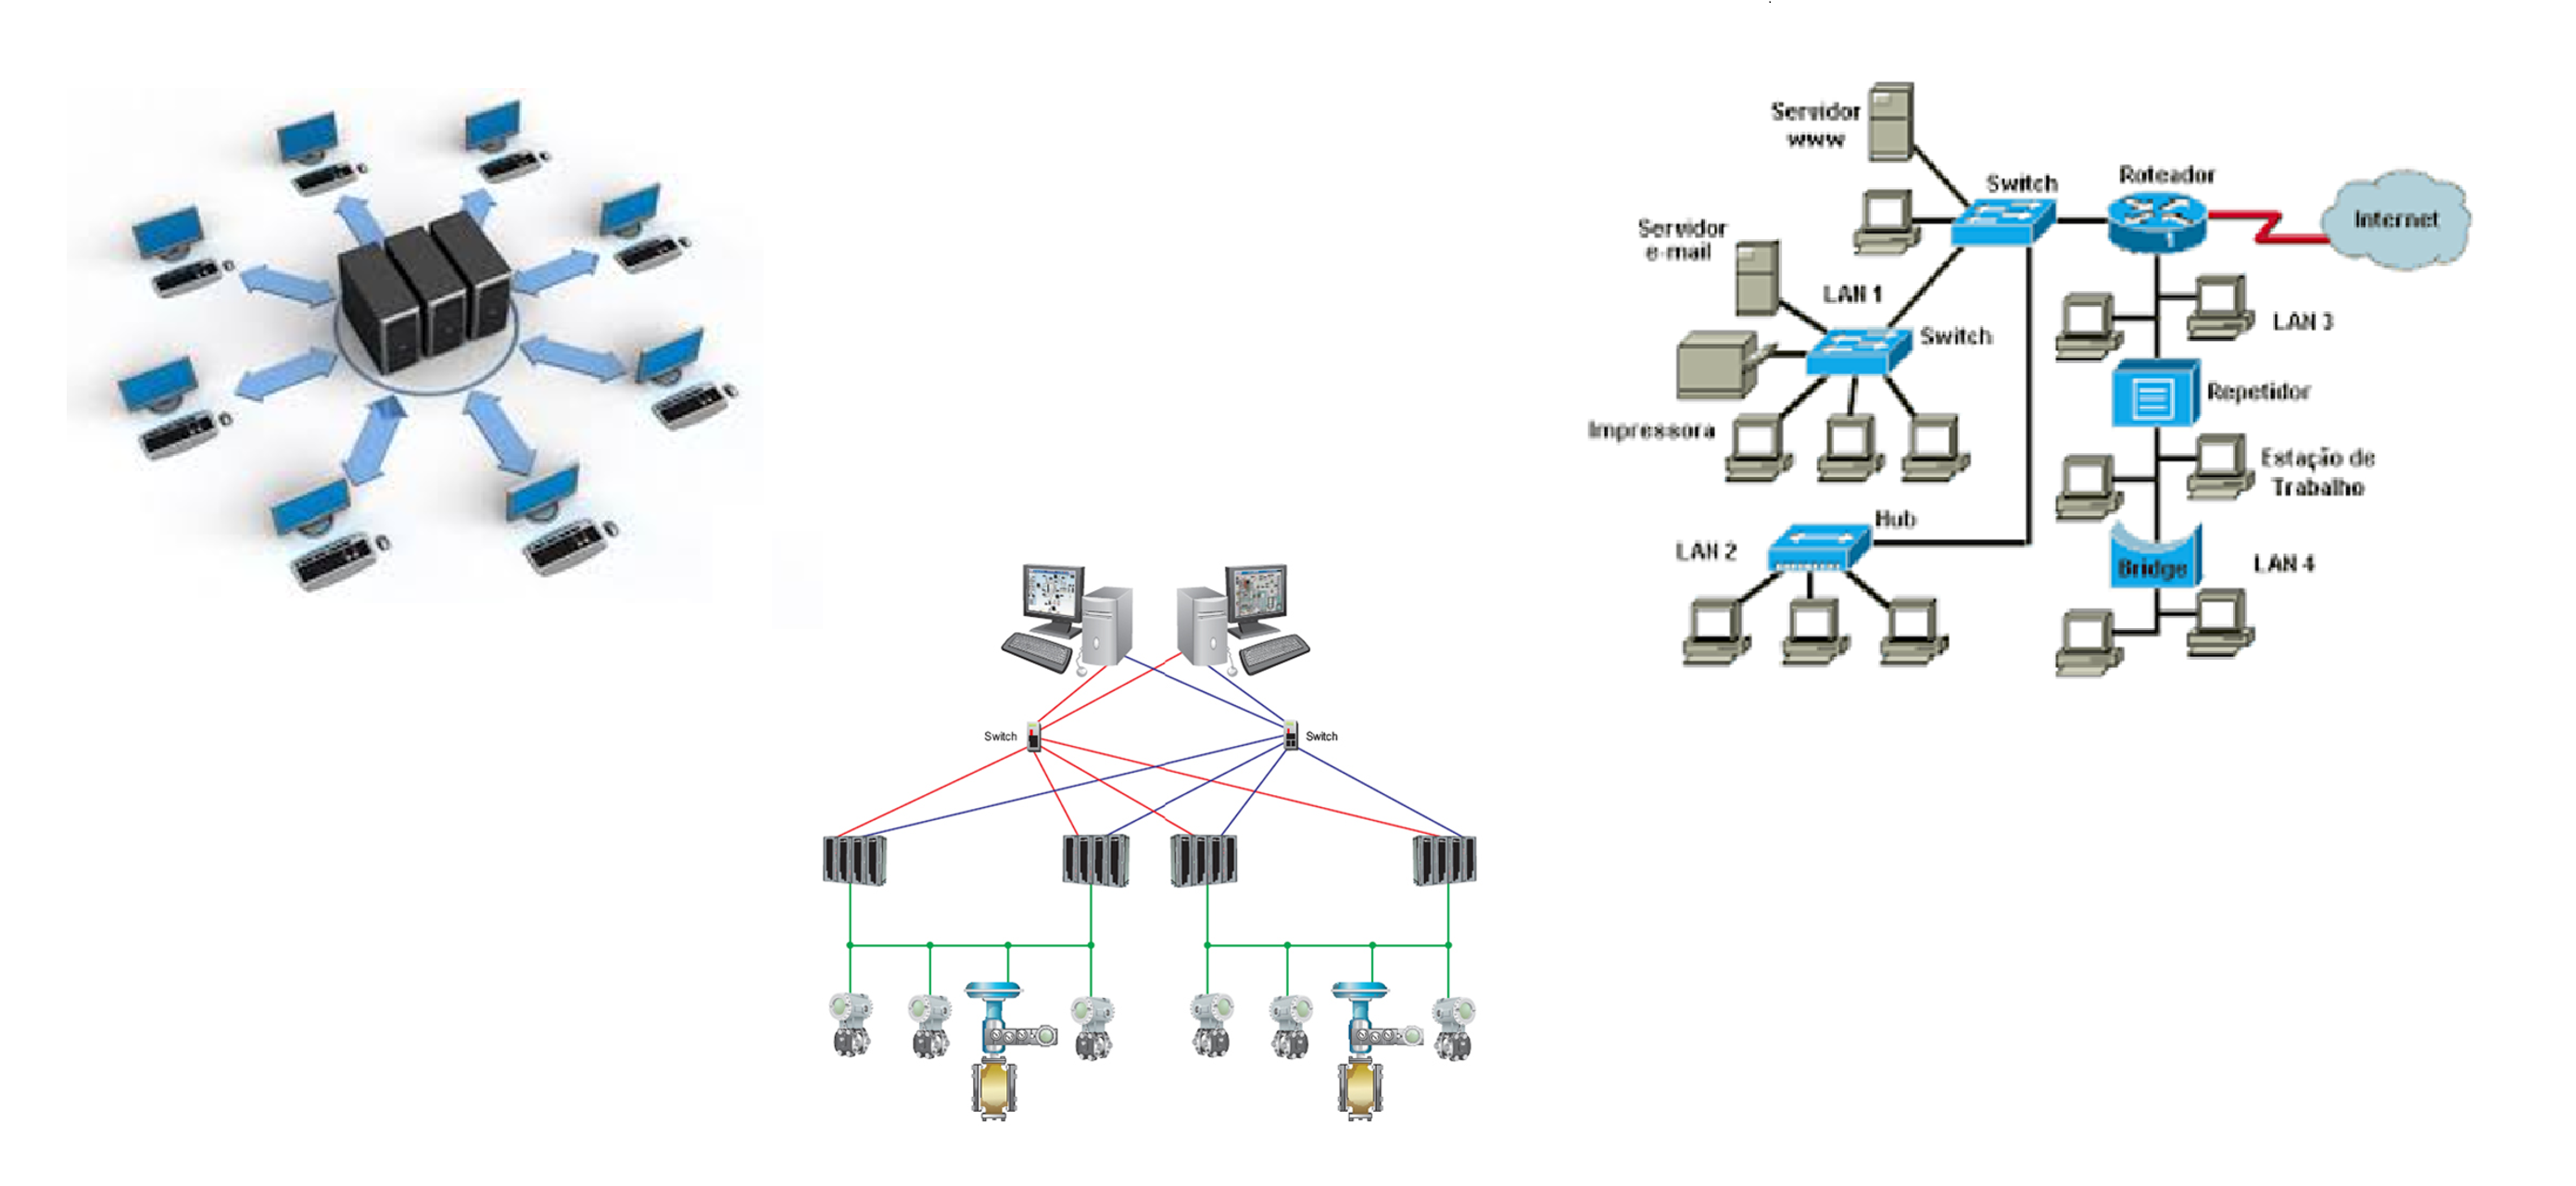
\includegraphics[height=5cm, keepaspectratio]{../figs/cap01/redes03.png} 
		\end{figure}
	\end{frame}		
	
	\begin{frame}
		\frametitle{Introdução}
		\begin{itemize}
			\item As redes surgiram da necessidade de compartilhar dados em tempo hábil.
			\item Os computadores pessoais são ferramentas de trabalho ótimas para produzir dados, gráficos e outros tipos de informação, mas não possibilitam que você compartilhe rapidamente os dados que criou.

		\end{itemize}
	\end{frame}	
		
	\begin{frame}
		\frametitle{Introdução}
		\begin{itemize}
			\item Um conjunto de computadores e outros dispositivos conectados juntos chama-se REDE, assim como o conceito de computadores compartilhando os recursos.
			\item Um computador conectado a outros pode compartilhar os dados dos outros computadores, impressoras e outros dispositivos.
		
		\end{itemize}
	\end{frame}
	
	\begin{frame}
		\frametitle{Compartilhamento}
		\begin{itemize}
			\item Os computadores que fazem parte de uma rede podem compartilhar
			\begin{itemize}
				\item Dados
				\item Mensagens
				\item Gráficos
				\item Impressoras
				\item Aparelhos de fax
				\item Modems
				\item Outros recursos de Hardware
			\end{itemize}
		\end{itemize}
	\end{frame}
	
	\begin{frame}{Sistema distribuído}
		\begin{itemize}
			\item Um \textcolor{red}{sistema distribuído} é aquele no qual os componentes localizados em \textcolor{red}{computadores} interligados em rede se \textcolor{red}{comunicam} e coordenam suas ações apenas passando \textcolor{red}{mensagens}.

		\end{itemize}
	\end{frame}
	
	\begin{frame}{Exemplos}
	
		\begin{figure}
			\centering
			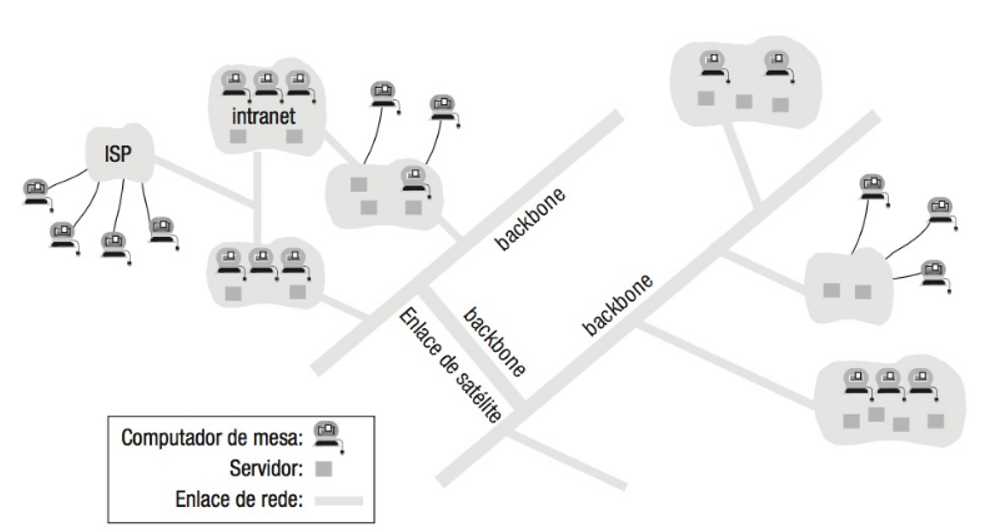
\includegraphics[height=.87\textheight, keepaspectratio]{../figs/cap01/sistemas2.png} 
		\end{figure}
	\end{frame}

	\begin{frame}{Exemplos}
	
		\begin{figure}
			\centering
			
\includegraphics[height=.87\textheight, keepaspectratio]{../figs/cap01/sistemas.png} 
		\end{figure}
	\end{frame}

	\begin{frame}{Sistemas distribuídos hoje}
		\begin{columns}[t]
			\begin{column}{0.5\textwidth}
				\begin{itemize}
					\item Internet of Things (IoT)
					\vspace{1em}
					\item Sistemas Multimídia 
					\begin{itemize}
						\item Spotify
						\item YouTube
						\item Netflix
					\end{itemize}
				\end{itemize}
			\end{column}
			\begin{column}{0.5\textwidth}
				\begin{itemize}
					\item Nuvem
					\begin{itemize}
						\item Execução de aplicativos
						\item Armazenamento
						\item Processamento Computacional
					\end{itemize}
					\vspace{1em}
					\item Computação móvel
					\vspace{1em}
					\item Grid Computing
				\end{itemize}
			\end{column}
		\end{columns}
	\end{frame}
	
	\begin{frame}{Termos importantes}
		\begin{itemize}
			\item \textbf{Serviço:} parte distinta de um sistema computacional que gerencia um conjunto de recursos relacionados e apresenta sua funcionalidade para usuários e aplicativos.
			\begin{itemize}
				\item Acesso limitado pelo conjunto de operações permitidas
				\item Evita que sejam feitas alterações indesejadas no sistema por pessoas não autorizadas
			\end{itemize}
		\end{itemize}
	\end{frame}

	\begin{frame}{Termos importantes}
		\begin{itemize}
			\item \textbf{Servidor:} Programa (processo) em execução em um nó da rede que aceita pedidos de execução de programas vindos de outros nós (clientes).
			\begin{itemize}
				\item Arquitetura cliente-servidor
				\item Podem ser implementados em forma de objetos
				\item Exemplos de utilização de arquitetura cliente-servidor
				\begin{itemize}
					\item WWW
					\item Email
					\item Impressoras
				\end{itemize}
			\end{itemize}
		\end{itemize}

	\end{frame}	
	
	\section{Características de Sistemas Distribuídos}

	\begin{frame}{Características de Sistemas Distribuídos}
		\begin{itemize}
			\item Concorrência de componentes
			\begin{itemize}
				\item Realização de uma tarefa por diversas máquinas
			\end{itemize}
			\vspace{1em}
			\item Falta de um relógio global 
			\begin{itemize}
				\item Podem gerar falhas devido à falta de sincronização
			\end{itemize}
			\vspace{1em}
			\item Falhas de componentes independentes.
			\begin{itemize}
				\item Podem ocorrer de forma isolada, porém afetando toda a rede
			\end{itemize}
		\end{itemize}
	\end{frame}
	
	\section{Desafios de implementação}
	\begin{frame}{Desafios de implementação}
		\begin{itemize}
			\item Heterogeneidade
			\vspace{1em}
			\item Sistemas abertos
			\vspace{1em}
			\item Segurança
			\vspace{1em}
			\item Estabilidade
			\vspace{1em}
			\item Tratamento de falhas
			\vspace{1em}
			\item Transparência
		\end{itemize}
	\end{frame}

	\begin{frame}{Heterogeneidade}
		\begin{itemize}
			\item Diferença entre os computadores e redes que executam os processos
			\vspace{1em}
			\item Aplicável a
			\begin{itemize}
				\item Redes
				\item Hardware
				\item Sistemas operacionais
				\item Linguagens de programação
				\item Implementação
			\end{itemize}
		\end{itemize}
	\end{frame}

	\begin{frame}{Middleware}
		\begin{itemize}
			\item Camada de software que oferece abstração de programação
			\vspace{1em}
			\item Trata das diferenças em nível dos sistemas operacionais e do hardware 
			\vspace{1em}
			\item Exemplos
			\begin{itemize}
				\item CORBA (\textit{Common Object Request Broker})
				\item JAVA RMI
			\end{itemize}
		\end{itemize}
	\end{frame}
	
	\begin{frame}{Middleware - Funcionalidades}
		\begin{itemize}
			\item Invocação remota de objetos
			\vspace{1em}
			\item Notificação de eventos
			\vspace{1em}
			\item Acesso a banco de dados
			\vspace{1em}
			\item Processamento de transação 
		\end{itemize}
	\end{frame}
	
	\begin{frame}{Sistemas abertos}
		\begin{itemize}
			\item Oferecem a possibilidade de extensão e reimplementação de funções do sistema
			\begin{itemize}
				\item Recompilar o kernel
			\end{itemize}
			\vspace{1em}
			\item Em geral utilizam licenças que permitem a alteração do código pelos desenvolvedores sem nenhum custo (GPL, LGPL)
		\end{itemize}
	\end{frame}
	
	\begin{frame}{Segurança}
		\begin{itemize}
			\item Certos dados devem ser mantidos de forma confidencial no sistema, permitindo acesso apenas ao pessoal autorizado
			\vspace{1em}
			\item Componentes de segurança
			\begin{itemize}
				\item Confidencialidade
				\item Integridade
				\item Disponibilidade
			\end{itemize}
		\end{itemize}
	\end{frame}

	\begin{frame}{Escalabilidade}
		\begin{itemize}
			\item Manutenção da eficiência do serviço com o aumento do número de usuários
			\vspace{1em}
			\item Desafios
			\begin{itemize}
				\item Controle de custos
				\item Perda de desempenho
				\item Esgotamento de recursos
				\item Gargalos de desempenho
			\end{itemize}
		\end{itemize}
	\end{frame}
	
	\begin{frame}{Concorrência}
		\begin{itemize}
			\item Compartilhamento de recursos pelos clientes pode ocasionar o acesso simultâneo
			\vspace{1em}
			\item Exige sincronização para manutenção da consistência
		\end{itemize}
	\end{frame}
	
	\begin{frame}{Transparência}
		\begin{itemize}
			\item Visão do sistema como um todo pelo usuário, sem necessidade de conhecimento dos componentes
			\vspace{0.8em}
			\item Tipos
			\begin{itemize}
				\item Acesso
				\item Localização
				\item Concorrência
				\item Replicação
				\item Falhas
				\item Mobilidade
				\item Desempenho
				\item Escalabilidade
			\end{itemize}
		\end{itemize}
	\end{frame}

	\begin{frame}{}
	\end{frame}
	
\end{document}
